\begin{theorem}
	\hypertarget{thrm5.7}{(Инвариантность формы первого дифференциала и неинвариантность формы высших дифференциалов)} Пусть функция $y = y(x)$ дифференцируема в точке $x_{0},$ а функция $z = z(x)$ дифференцируема в точке $y_{0} = y(x_{0}).$
	
	Тогда дифференциал $z,$ рассматриваемый как функция лишь от $y$ в точке $y_{0},$  и дифференциал функции $z= z(y(x)) = f(x)$ в точке $x_{0}$ записываются одинаково. А именно $dz = z'(y_{0}) \ dy$. При этом в первом случае (когда $z=z(y)$) $dy = y-y_{0}$, а во втором $dy$~---~ дифференциал функции $y(x)$ в точке $x_{0}$
\end{theorem}
\begin{proof}
	Для функции $z = z(y)$ по определению дифференциала 
	
	$$dz(y_{0}) = z'(y_{0}) \ dy, \ dy = y-y_{0}$$
	
	Рассмотрим композицию функций $z = z(y(x)) = f(x)$.
	
	$$dz = f'(x_{0}) \ dx = z'(y(x_{0})) \ y'(x_{0}) \ dx = z'(y(x_{0})) \ dy(x_{0})$$
\end{proof}

\begin{note}
	Для второго дифференциала форма записи не инвариантна.
\end{note}
\begin{proof}
	Действительно, пусть функция $z = z(y)$ дважды дифференцируема в точке $y_{0}$
	
	$$d^{2} = z''(y_{0}) \ (dy)^{2}, \ dy = y-y_{0}$$
	
	Если же $z = z(y(x))$
	
	$$d^{2} z = f''(x_{0}) \ (dx)^{2} = \Bigl( z'(y(x)) \cdot y'(x) \Bigr)' \ (dx)^{2}, \Big|_{x = x_{0}}
	$$
	
	$$
	= \Bigl[z''(y(x)) \cdot (y'(x))^{2} + z'(y(x))\cdot y''(x_{0}) \Bigr] \cdot (dx)^{2} = z''(y_{0}) \cdot (y'(x_{0}))^{2} \cdot (dx)^{2} + z'(y(x_{0})) \cdot y''(x_{0}) \cdot (dx)^{2} =$$
	
	$$
	= z''(y_{0}) (dy)^2 + z'(y_{0}) \ d^{2} y(x_{0})
	$$
\end{proof}

\subsection{Формула Лейбница}
Введём некоторые обозначения: 
$$0! :=1$$
$$ n! := 1 \cdot 2 \cdot \ldots \cdot n, \quad n \in \N $$

$ \relax C_{n}^{k}$~---~ биномиальный коэффициент.
$$ \relax C_{n}^{k} := \cfrac{n!}{k!(n-k)!}$$

Соглашение: $u^{(0)}(x) \equiv u(x)$

\begin{theorem} \hypertarget{thrm5.8}{Формула Лейбница}
	Пусть $\exists u^{(n)}(x_{0}) \in \R $ и $\exists v^{(n)}(x_{0}) \in \R$
	
	Тогда $\exists (u\cdot v)^{n} = \sum\limits_{s=0}^{n} \relax C_{n}^{s} u^{(s)}(x_{0}) \cdot v^{(n-s)}(x_{0})$
\end{theorem}
\begin{proof}
	Докажем по индукции.
	
	База индукции: при $n =1 $ верно (\hyperlink{thrm5.3}{обычное правило дифференцирование произведения}).
	
	Пусть доказано при некотором $k \in \N,$ установим при $k + 1$
	
	То есть мы доказали формулу при $k \in \N$:
	$$(u \cdot v)^{(k)} = \sum\limits_{s=0}^{k} \relax C_{k}^{s} u^{(s)}(x_{0}) \cdot v^{(k-s)}(x_{0}) $$
	
	$$
	(u \cdot v)^{(k+1)} = \Bigg(\sum\limits_{s=0}^{k} \relax C_{k}^{s} u^{(s)}(x) \cdot v^{(k-s)}(x) \Bigg)' \Bigg|_{x=x_{0}} = 
	$$
	$$ =\sum\limits_{s=0}^{k} \relax C_{k}^{s} u^{(s+1)}(x_{0}) \cdot v^{(k-s)}(x_{0}) + \sum\limits_{s=0}^{k} \relax C_{k}^{s} u^{(s)}(x_{0}) \cdot v^{(k-s + 1)}(x_{0}) = (*)
	$$
	Произведем замену индексов: $ s + 1 = j, \ s+ j - 1$
	$$
	(*) = \sum\limits_{j=1}^{k+1} \relax C_{k}^{j-1} u^{(j)}(x_{0}) \cdot v^{(k-j + 1)}(x_{0}) + \sum\limits_{j=0}^{k} \relax C_{k}^{j} u^{(j)}(x_{0}) \cdot v^{(k-j + 1)}(x_{0}) =
	$$
	
	$$
	=  \relax C_{k}^{k} u^{(k+1)}(x_{0}) \cdot v(x_{0}) + \relax C_{k}^{0} u(x_{0}) \cdot v^{(k+ 1)}(x_{0}) + \sum\limits_{j=1}^{k} \Bigl(\relax C_{k}^{j-1} + \relax C_{k}^{j} \Bigr) u^{(j)}(x_{0}) \cdot v^{(k+1 -j)}(x_{0}) = 
	$$
	
	Заметим, что
	
	$
	\relax C_{k}^{k} = \relax C_{k+1}^{k+1} = 1,$
	
	$\relax C_{k}^{0} = \relax C_{k + 1}^{0} = 1,
	$
	
	$
	\relax C_{k}^{j-1} +  \relax C_{k}^{j} = \cfrac{k!}{(j-1)!(k-j + 1)!} + \cfrac{k!}{(j)!(k-j)!} =
	$
	$$
	= \cfrac{k!}{(j)!(k-j+1)!} \cdot ( k -j + 1 + j) = \cfrac{(k+1)!}{(j)!(k+1-j)!} = C_{k+1}^{j}
	$$
	
	С учетом этого перепишем выражение $(*)$
	
	$$
	(u \cdot v)^{(k+1)} = (*) = \sum\limits_{j=0}^{k+1} \relax C_{k+1}^{j} u^{(j)}(x_{0}) \cdot v^{(k+1-j)}(x_{0})
	$$
	
	Шаг индукции доказан. Значит, формула верна при всех $n \in \N.$
\end{proof}

\subsection{Вычисление производных функций, заданных неявно}

\begin{definition}
	Будем говорить, что функция $y: X \mapsto \R$ \textit{неявно задана уравнением} $F(x, y) = 0$, если $F(x,y(x)) = 0 \quad \forall x \in X$  
\end{definition}
\begin{example}
	$$x^2 + y^2 = 1$$
	$$F (x, y) = x^2 + y^2 - 1 $$
	
	$y_{1}(x) = \sqrt{1-x^2}$~---~ функция, неявно заданная уравнением $F (x, y) = 0$
	
	$y_{2}(x) = -\sqrt{1-x^2}$~---~ функция, неявно заданная уравнением $F (x, y) = 0  $
	
	Также заметим, что функций, неявно задающихся данным уравнением, бесконечно много.
\end{example}

\begin{note}
	В домашних задачах априори предполагается, что неявно заданные функции существуют и они дифференцируемы. Однако в общем случае это нужно доказывать.
\end{note}

Чтобы найти производную неявно заданной функции, необходимо:
\begin{enumerate}
	\item Продифференцировать обе части уравнения, вместо $y$ подставляя $y(x)$. Так как оно является тождеством при всех значениях $x$,
	\item Выразить производную $y'(x)$.
\end{enumerate}

\subsection{Производные функций, заданных параметрически}
Пусть $\begin{gathered}
	y = y(t), \\
	x = x(t)
\end{gathered}$ определены в некоторой $U_{\delta}(t_{0})$. 

Если для $x$ выполнены условия, требуемые для \hyperlink{thrm4.19}{теоремы об обратной функции}, то $\exists t = t(x),$ определенная в $U_{delta}(x_{0}),\ x_{0} = x(t_{0})$.

Пусть также выполнены все условия \hyperlink{5.11}{ теоремы о дифференцировании обратной функции} и \hyperlink{thrm5.10}{теоремы о дифференцировании сложной функции}. Тогда

$$f(x) = y(t(x))$$

$$y'_{x}(x_{0}) = \cfrac{y'_{t}(t_{0})}{x'_{t}(t_{0})}, \textrm{где} \ t_{0} = t(x_{0})$$

\subsection{Теоремы о среднем}

\begin{definition}
	Пусть $f : X \mapsto \R, X \subset \R$.
	
	Будем говорить, что точка $x_{0}$~---~ \textrm{точка локального максимума (локального минимума) функции $f$, то есть, точка локального экстремума,} если 
	$$\exists \delta = \delta (x_{0}) > 0: \begin{gathered}
		f(x) \leq f(x_{0}) \ \forall x \in U_{\delta}(x_{0}) \cap X\\
		\Bigl( f(x) \geq f(x_{0}) \ \forall x \in U_{\delta}(x_{0}) \cap X\Bigr) 
	\end{gathered}$$
\end{definition}

\begin{definition}
	Пусть $f : X \mapsto \R, X \subset \R$.
	
	Будем говорить, что точка $x_{0}$~---~ \textrm{точка строгого локального максимума (строгого локального минимума), то есть строгого экстремума функции $f$,} если 
	$$\exists \delta = \delta (x_{0}) > 0: \begin{gathered}
		f(x) < f(x_{0}) \ \forall x \in \mathring{U}_{\delta}(x_{0}) \cap X\\
		\left( f(x) > f(x_{0}) \ \forall x \in \mathring{U}_{\delta}(x_{0}) \cap X\right) 
	\end{gathered}$$
\end{definition}

\begin{lemma}
	Пусть $f: [a, b] \mapsto \R$. Пусть $x_{0}$~---~ точка локального минимума (локального максимума).
	
	Тогда, если $ \begin{gathered}
		\exists f'_{+} (x_{0}), \textrm{то}  f'_{+} (x_{0}) \geq 0 \\
		\exists f'_{-} (x_{0}), \textrm{то}  f'_{-} (x_{0}) \leq 0 \\
		\left(
		\begin{gathered}
			\exists f'_{+} (x_{0}), \textrm{то} f'_{+} (x_{0}) \leq 0 \\
			\exists f'_{-} (x_{0}), \textrm{то} f'_{-} (x_{0}) \geq 0			
		\end{gathered}
		\right)
	\end{gathered}$
\end{lemma}
\begin{proof}
	.
	
	\sidefig(10 cm)(7 cm)	
	{\begin{flushleft}
			
			Докажем для случая, когда $x_{0}$~---~ точка локального минимума, так как для локального максимума доказательство аналогично.	
			
			Пусь $ \exists f'_{+}(x_{0}) \Rightarrow \exists \lim\limits_{x\to x_{0}+0} \cfrac{f(x)-f(x_{0})}{x - x_{0}}$
			
			Так как $x_{0}$~---~ локальный максимум, то
			
			$$\exists \delta > 0: \ f(x)\geq f(x_{0}) \quad \forall x\in U_{\delta}(x_{0}) \cap [a,b]$$
			
			А так как берется правсторонний предел, то $x>x_{0}$. Следовательно,
			$\forall x \in \mathring{U}^{+}_{\delta} (x_{0}) \cap [a, b] \hookrightarrow \cfrac{f(x)-f(x_{0})}{x-x_{0}} \geq 0 
			$
			
		\end{flushleft}
	}
	{
		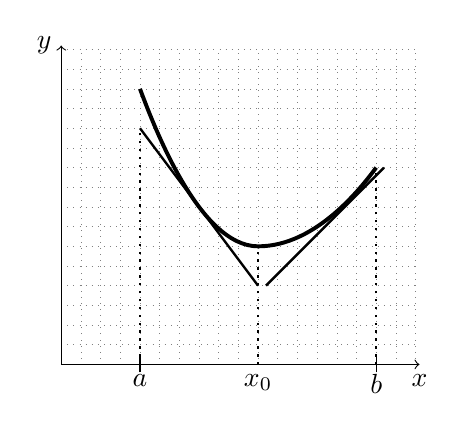
\begin{tikzpicture}
			% Рисуем сетку
			\draw[help lines, step=0.25, dotted]
			(0,0) grid (4.5,4);
			% Начало координат
			\draw[->, thin] (0,0) -- (4.55,0)
			node[below] {$x$}; % Ox
			\draw[->, thin] (0,0) -- (0, 4.05)
			node[left] {$y$}; % Oy
			
			\draw[line width =.05cm](1, 3.5) parabola bend (2.5, 1.5)(4, 2.5);
			
			\draw[line width =.03cm] (1, 3) -- (2.5, 1);
			\draw[line width =.03cm] (2.6, 1) -- (4.1, 2.5);
			
			\draw[dotted, line width =.03cm] (2.5, 0) -- (2.5, 1.5);
			\draw[dotted, line width =.03cm] (1, 0) -- (1, 3);
			\draw[dotted, line width =.03cm] (4, 0) -- (4, 2.5);
			
			\node[below] at (1, 0) {$a$};
			\node[below] at (2.5, 0) {$x_{0}$};
			\node[below] at (4, 0) {$b$};
			
			\draw[thin] (1, -0.1) -- (1, 0.1);
			\draw[thin] (4, -0.1) -- (4, 0.1);
		\end{tikzpicture}
	}
	
	Следовательно, делая \hyperlink{thm4.8}{предельный переход в неравенстве}, получим $f'_{+} \geq 0$
	
	Если $\exists f'_{-}(x_{0}) := \lim\limits_{x\to x_{0}-0} \cfrac{f(x)-f(x_{0})}{x-x_{0}}$, то
	$ \exists \delta > 0: \ f(x) \geq f(x_{0}) \quad \forall x\in U_{\delta}(x_{0})
	$
	
	Так как $x$ приближается к $x_{0}$ слева, то $x-x_{0} \leq 0$. Следовательно,
	
	$$\forall x \in \mathring{U}^{-}_{\delta} (x_{0}) \cap [a, b] \hookrightarrow \cfrac{f(x)-f(x_{0})}{x-x_{0}} \leq 0
	$$
	
	Следовательно, делая \hyperlink{thm4.8}{предельный переход в неравенстве}, получим $f'_{-} \leq 0$
\end{proof}

\begin{theorem}
	\hypertarget{thrm6.1}{(Теорема Ферма)} Пусть $f: \ U_{\delta}(x_{0}) \mapsto \R$ дифференцируема в точке $x_{0}$. Тогда, если $x_{0}$~---~ локальный экстремум $f$, $f'(x_{0}) = 0$
\end{theorem}
\begin{proof}
	В силу предыдущей леммы $ \begin{cases}
		f'_{+}(x_{0}) \geq 0 \\
		f'_{-}(x_{0}) \leq 0,
	\end{cases}$
	если $x_{0}$~---~ локальный минимум. Следовательно, $\exists f'(x_{0}) \in \R \Leftrightarrow \begin{cases}
		\exists f'_{+}(x_{0}) \in \R \\
		\exists f'_{-}(x_{0}) \in \R
	\end{cases}$
	и $f'_{+}(x_{0}) = f'_{-}(x_{0}) \Rightarrow f'(x_{0}) = 0.$
	
	Доказательство для локального максимума аналогично.
\end{proof}

\begin{theorem}
	\hypertarget{thrm6.2}{Ролля (о среднем)} Пусть $f \in C([a,b])$ и дифференцируема на интервале. 
	
	Пусть значения на концах равна, тогда $\exists \xi \in (a, b): f'(\xi) = 0.$
\end{theorem}
\begin{proof}
	Возможны два случая:
	
	$\underline{\textrm{Случай 1}}$ $f \equiv const. \ f'(x) = 0 \quad \forall x\in (a, b)$
	
	Значит, в качестве $\xi$ можно взять любую точку из $(a, b)$
	
	$\underline{\textrm{Случай 2}}$ Если $f \neq const,$ то в силу непрерывности $f$ достигает наибольшего и наименьшего значения на $[a, b].$
	
	Следовательно, $\exists$ точка локального экстремума $\xi \in [a,b]$ (в котором достигается либо локальный максимум, либо локальный минимум)
	
	Значит, так как $f$ дифференцируема на интервале $(a, b)$, по \hyperlink{thrm6.1}{теореме Ферма} $f'(\xi) = 0$
\end{proof}

\begin{theorem}
	\hypertarget{thrm 6.3}{Коши (о среднем)} Пусть $f,g \in C([a, b])$и дифференцируема на интервале $(a, b)]$. Пусть $g'(x) \neq 0 \quad \forall x \in (a, b).$ 
	
	Тогда $\exists \xi \in (a, b): \ \cfrac{f(b)-f(a)}{g(b)-g(a)}= \cfrac{f'(\xi)}{g'(\xi)} $ 
\end{theorem}
\begin{proof}
	Так как $g'(x) \neq 0 \quad \forall x \in [a, b],$ То $g(a) \neq g(b)$. Иначе получили противоречие \hyperlink{thrm6.2}{теореме Ролля}. Следовательно, формула корректна.
	
	Рассмотрим функцию $h(x) = f(x) - kg(x), \textrm{при}\ k =\cfrac{f(b)-f(a)}{g(b)-g(a)}.$
	
	Заметим, что $h(b) =h(a)$.
	
	$h \in C([a,b])$ и дифференцируема на интервале $(a, b)$. По \hyperlink{thrm6.2}{теореме Ролля} $$\exists \xi \in (a, b): h'(\xi) = 0$$
	
	$h'(\xi) = f'(\xi) - k g'(\xi) = 0 \Rightarrow k = \cfrac{f'(\xi)}{g'(\xi)} \Rightarrow \cfrac{f(b)-f(a)}{g(b)-g(a)}= \cfrac{f'(\xi)}{g'(\xi)}$
\end{proof}


\sidefig(10 cm)(7 cm)	
{\begin{flushleft}
		Предположим, что на малом интервале $x(t)$ обратима и удволетворяет условиям \hyperlink{thrm4.19}{теоремы об обратной функции}
		$$
		\begin{gathered}
			x = x(t) \\
			y = y(t)
		\end{gathered} \quad \quad
		y'(x) = \cfrac{y'(t)}{x'(t)}\Bigg|_{t = t(x)}
		$$
	\end{flushleft}
}
{
	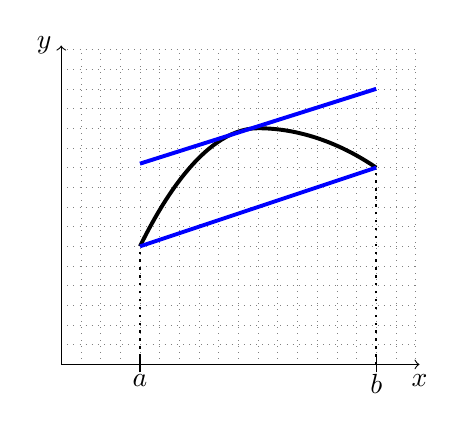
\begin{tikzpicture}
		% Рисуем сетку
		\draw[help lines, step=0.25, dotted]
		(0,0) grid (4.5,4);
		% Начало координат
		\draw[->, thin] (0,0) -- (4.55,0)
		node[below] {$x$}; % Ox
		\draw[->, thin] (0,0) -- (0, 4.05)
		node[left] {$y$}; % Oy
		
		\draw[line width =.05cm](1, 1.5) parabola bend (2.5, 3)(4, 2.5);
		
		\draw[line width =.05cm, blue] (1, 1.5) -- (4, 2.5);
		\draw[line width =.05cm, blue] (1, 2.55) -- (4, 3.5);
		
		\draw[dotted, line width =.03cm] (1, 0) -- (1, 1.5);
		\draw[dotted, line width =.03cm] (4, 0) -- (4, 2.5);
		
		\node[below] at (1, 0) {$a$};
		\node[below] at (4, 0) {$b$};
		
		\draw[thin] (1, -0.1) -- (1, 0.1);
		\draw[thin] (4, -0.1) -- (4, 0.1);
	\end{tikzpicture}
}

\begin{corollary}
	\hypertarget{thrm6.4}{(Теорема Лагранжа о среднем)} Пусть $f \in C([a, b])$ и дифференцируема на интервале $(a, b)$.
	
	Тогда найдется $\xi \in (q, b): \ f(b) - f(a) = f'(\xi)(b-a)$
\end{corollary}
\begin{proof}
	Применить теорему Коши о среднем при $f = f$ и $g = x$
\end{proof}

\subsection{Следствия из теоремы Лагранжа о среднем}

\begin{theorem}
	Пусть $f \in C(U_{\delta}(x_{0})) $ Пусть $f$ дифференцируема в $\mathring{U}_{\delta}(x_{0})$
	
	Если $\exists \lim\limits_{x \to x_{0}+0} f'(x_{0}),$ то $\exists f'_{+}(x_{0)} = \lim\limits_{x\to x_{0}+0} f'(x)$
	
	Если $\exists \lim\limits_{x \to x_{0}-0} f'(x_{0}),$ то $\exists f'_{-}(x_{0}) = \lim\limits_{x\to x_{0}-0} f'(x)$
\end{theorem}
\begin{proof}
	Докажем для правой производной, так как для левой аналогично.
	
	Фиксируем $x\in \mathring{U}^{+}_{\delta}(x_{0})$. Выполнены все условия теоремы Лагранжа о среднем на отрезке $[x_{0}, x] \Rightarrow \xi(x) \in (x_{0}, x):\  \cfrac{f(x) - f(x_{0})}{x-x_{0}} = f'(\xi(x)) \quad (*)$
	
	$x$ был выбран произвольно, $\xi(x) \neq x_{0} \quad \forall x \in \mathring{U}^{+}_{\delta}(x_{0}) \Rightarrow $
	$$\Rightarrow \exists \lim\limits_{x \to x_{0}+0} f'(\xi(x)) =\lim\limits_{\xi \to x_{0}+0} f'(\xi) \Leftrightarrow \exists \lim\limits_{x \to x_{0}+0} \cfrac{f(x) - f(x_{0})}{x-x_{0}} = f'_{+}(x_{0})$$
	
	Значит, в силу $(*)$ получаем
	$
	\lim\limits_{\xi \to x_{0}+0} f'(\xi) = f'_{+}(x_{0})
	$
	
	Аналогично для левосторонней производной.
\end{proof}

\begin{corollary}
	Если $f$ дифференцируема на интервале $(a, b),$ то $f'$ не имеет разрывов 1-ого рода и устранимых разрывов.
\end{corollary}
\begin{proof}
	Из следствия теоремы Лагранжа о среднем вытекает, что если $\exists \lim\limits_{x\to x_{0}} f'(x),$ то он обязан быть равен $f'(x_{0})$. Значит, устранимых разрывов быть не может.
	
	При разрыве 1-ого рода односторонние пределы существуют, но не равны. Из следствия теоремы Лагранжа это значит, что существует првосторонняя и левостороняя призводная, но они не равны. Но это противоречит условию, что $f$ дифференцируема на $(a, b)$. Значит, $f'$ не имеет разрывов 1-ого рода. 
	
\end{proof}

Таким образом, если функция дифференцируема на интервале $(a,b)$, то разрывы у нее могут быть только второго рода. 

\begin{example}
	$f(x) = \begin{cases}
		x^2 \cdot \sin \cfrac{1}{x}, x\neq 0 \\
		0, x = 0 \hfill
	\end{cases}$
	
	$f$ дифференцируема всюду на $\R$, но производная имеет разрыв второго рода
\end{example}
\begin{proof}
	Если $x\neq 0$, то $f'(x) = 2x \cdot\sin \cfrac{1}{x} + x^{2} \cos \cfrac{1}{x} \cdot \left(\cfrac{-1}{x^2}\right) = 2x\cdot\sin \cfrac{1}{x} - \cos \cfrac{1}{x} $
	
	$$f'(0) = \lim\limits_{x\to 0} \cfrac{f(x) - f(0)}{x} = \lim\limits_{x\to 0} \cfrac{x^2\cdot \sin \cfrac{1}{x} - 0}{x} =  \lim\limits_{x\to 0} x \sin \cfrac{1}{x} = 0$$
	
	$\nexists \lim\limits_{x\to 0} f'(x) \Rightarrow \ f'$ имеет в нуле разрыв второго рода 
\end{proof}

\subsection{Теорема Дарбу}

\begin{lemma}
	Пусть $f$ дифференцируема на интервале $(a, b)$. 
	
	Пусть $x, y \in (a, b)$ и $f'(x) \cdot f'(y) < 0$. Тогда $\exists \xi \in (x, y):\  f'(\xi) = 0$
\end{lemma}
\begin{proof}
	Рассмотрим случай $f'(x) > 0 \ f'(y) < 0$. Так как $f \in C((a, b)) \Rightarrow f \in C([x,y])$. Значит, $ f$ достигает максимума и минимума на $[x,y].$ Точка максимума находится на $(x,y)$, так как $\begin{cases}
		f'_{+}(x_{M}) \leq 0\\
		f'_{-}(x_{M}) \geq 0
	\end{cases}$. То есть точка максимума $\begin{cases}
		x_{M} \neq x,\\
		x_{M} \neq y.
	\end{cases}$
	
	Следовательно, \hyperlink{thrm6.1}{по теореме Ферма} $f'(x_{M}) = 0.$
	
	Аналогично рассматривается случай $f'(x) < 0 \ f'(y) > 0$.
\end{proof}

\begin{theorem}
	\hypertarget{thrm6.5}{(Теорема Дарбу)} Пусть $f$ дифференцируема на интервале $(a, b)$. Тогда если $f'$ принимает какие-либо два значения, то она принимает все значения между ними.  
\end{theorem}
\begin{proof}
	$\begin{cases}
		f'(x) = A \\
		f'(y) = B \\
		A \neq B
	\end{cases}$ Покажем, что $\forall C\in \left(A, B\right) \ \exists x_{c} \in (x,y): f'(x_{c}) = C $
	
	Фиксируем $C \in \left(A, B \right)$. Рассмотрим $h(t) = f(t) - C\cdot t$.
	
	$h$ дифференцируема на $(x,y)$. 
	
	$$\begin{gathered}
		h'(x) = f'(x) - C = A - C \\
		h'(y) = f'(y) - C = B-C
	\end{gathered}
	\Rightarrow h'(x)\cdot h'(y) = \left(A-C\right)\left(B-C\right) < 0 $$
	
	Следовательно, по предыдущей лемме:
	
	$$\exists \xi \in (x,y): \ h'(\xi) = 0 = f'(\xi) - C \Rightarrow f'(\xi) = 0$$
	
	Тогда положим $x_{c} = \xi$
\end{proof}

\subsection{Формула Тейлора}

\begin{definition}
	Пусть $n \in \N_{0},$ $f: U_{\delta}(x_{0})\mapsto \R$ имеет n-ую (конечную) производную в точке $x_{0}$. Тогда \textit{полиномом (многочленом) Тейлора функции $f$ с центром в точке $x_{0}$} называется
	
	$$T_{x_{0}}^{n} [f](x) := \sum\limits_{k = 0}^n \cfrac{f^{(k)}}{k!}(x-x_{0})^{k}.$$ 
\end{definition}

\begin{definition}
	\textit{Формальным n-ым остаточным членом формулы Тейлора функции $f$ с центром в точке $x_{0}$} называется 
	
	$$r_{x_{0}}^{n} [f](x):= f(x) -T_{x_{0}}^{n} [f](x),\ x\in U_{\delta_{0}}(x_{0}) $$
\end{definition}

\begin{lemma}
	$\phi_{n}(x) = (x-x_{0})^{n}$ Тогда 
	\begin{enumerate} 
		\item[a)] $\forall k \in \{0, \ldots, n\} \hookrightarrow \phi_{n}^{(k)} = n(n-1)\ldots (x-k+1)(x-x_{0})^{n-k}, $
		
		$ \forall k> n \hookrightarrow \phi_{n}^{(k)}(x) \equiv 0$
		\item[b)] $\phi_{n}^{(k)}(x_{0}) = \begin{cases}
			0, k \neq n\\
			n!, k =n
		\end{cases}$
	\end{enumerate}
\end{lemma}
\begin{proof}
	Пункт b) сразу следует из пункта  a)
	
	Пункт a) доказывается по индукции:
	
	При $k = 1$ очевидно.
	
	Пусть доказано при каком-то $k \in \N, \ k \in \{1, \ldots, n-1\}$
	
	Тогда $\Bigl((x_{0})^{n}\Bigr)^{(k+1)} =\Bigl(n(n-1)\ldots(n-k+1)(x-x_{0})^{n-1}\Bigr)' =$
	
	$$= n(n-1)\ldots (x-k+1)(x-x_{0})^{n-(k+1)} $$
\end{proof}

\begin{lemma}
	Пусть $\exists f^{(n)}(x_{0}) \in \R$. Тогда $\forall k \in \{0, \ldots, n\} \hookrightarrow \Bigl(r_{x_{0}}^{n} [f](x) \Bigr)^{(k)}(x_{0}) = 0$
\end{lemma}
\begin{proof}
	Фиксируем $ k \in \{0, \ldots, n\}$
	
	$$r_{x_{0}}^{n} [f](x) = f(x_{0}) -  \sum\limits_{j = 0}^n \cfrac{f^{(j)}}{j!}(x-x_{0})^{j} $$
	
	$$\Bigl(r_{x_{0}}^{n} [f](x)\Bigr)^{(k)} \Big|_{x = x_{0}} = f^{(k)}(x_{0}) -  \Biggl(\sum\limits_{j = 0}^n \cfrac{f^{(j)}}{j!}(x-x_{0})^{j}\Biggr)^{(k)} \Bigg|_{x=x_{0}} = f^{(k)}(x_{0}) - f^{(k)}(x_{0}) \cfrac{k!}{k!} = 0
	$$
\end{proof}

\begin{theorem}
	\hypertarget{thrm7.1}{(Формула Тейлора с остаточным членом в форме Пеано)} Путь $f$ дифференцируемо в точке $x_{0} \ n$ раз, $n \in \N_{0.}$ Тогда 
	
	$$f(x) = \sum\limits_{k = 0}^n \cfrac{f^{(k)}}{k!}(x-x_{0})^{k} + o\Bigl( (x-x_{0})^{n} \Bigr), x \to x_{0}$$
	\begin{note}
		Запись $x\to x_{0}$ означает, что равенство справедливо в некоторой окрестности $U_{\delta}(x_{0})$
		
		$o\Bigl( (x-x_{0})^{n} \Bigr)$~---~ это <<функция>>, предстваимая в виде $$\epsilon_{x_{0}}[f](x)(x-x_{0})^{n}, \ \textrm{где} \ \epsilon_{x_{0}}[f](x) \to 0, x\to x_{0}.$$
	\end{note}	
	
\end{theorem}
\begin{proof}
	Так как $\exists f^{(n)}(x_{0}),$ то $\exists U_{\delta}(x_{0}),$ в которой определена $f^{(n-1)}(x).$
	
	По определению $r_{x_{0}}^{n} [f](x) = f(x_{0}) - T_{x_{0}}^{n} [f](x), \quad \phi_{n}(x) = (x-x_{0})^{n}$
	
	Достаточно доказать, что $\cfrac{r_{x_{0}}^{n} [f](x)}{(x-x_{0})^{n}} \to 0, x\to x_{0}$
	
	
	Заметим, что $\phi_{n}(x_{0}) = (x-x_{0})^{n} = 0, \quad r_{x_{0}}^{n} [f](x_{0}) = 0.$ Тогда 
	
	$$\cfrac{r_{x_{0}}^{n} [f](x)}{(x-x_{0})^{n}} = \cfrac{r_{x_{0}}^{n} [f](x) - r_{x_{0}}^{n} [f](x_{0})}{\phi_{n}(x) - \phi_{n}(x_{0})} $$
	
	Так как $r_{x_{0}}^{n} [f](x)$ дифференцируема $n$ раз, то можно применить \hyperlink{thrm6.3}{теорему Коши о среднем}:
	
	$$ \cfrac{r_{x_{0}}^{n} [f](x) - r_{x_{0}}^{n} [f](x_{0})}{\phi_{n}(x) - \phi_{n}(x_{0})} = \cfrac{\Big(r_{x_{0}}^{n} [f]\Big)'(\xi)}{\phi_{n}'(\xi)},\ \textrm{где}\ \xi \in (x, x_{0})
	$$
	
	По предыдущей лемме имеем $\forall k \in \{0, \ldots, n\} \hookrightarrow \Bigl(r_{x_{0}}^{n} [f](x) \Bigr)^{(k)}(x_{0}) = 0$ и 
	
	$$\forall k \in \{0, \ldots, n-1\} \hookrightarrow \phi_{n}^{(k)}(x_{0})=0$$
	
	$$\cfrac{\Big(r_{x_{0}}^{n} [f]\Big)'(\xi)}{\phi_{n}'(\xi)} =\cfrac{r_{x_{0}}^{n-1} [f'](\xi)}{n \cdot \phi_{n-1}(\xi)} = \cfrac{\Big(r_{x_{0}}^{n} [f]\Big)'(\xi_{1}) - \Big(r_{x_{0}}^{n} [f]\Big)'(x_{0})}{n(\phi_{n-1}(\xi_{1}) - \phi_{n-1}(x_{0}))} $$
	
	Тогда, снова применяя \hyperlink{thrm6.3}{теорему Коши о среденем} получаем:
	$$
	\cfrac{\Big(r_{x_{0}}^{n} [f]\Big)'(\xi_{1}) - \Big(r_{x_{0}}^{n} [f]\Big)'(x_{0})}{n(\phi_{n-1}(\xi_{1}) - \phi_{n-1}(x_{0}))} = \cfrac{\Big(r_{x_{0}}^{n} [f]\Big)^{(2)}(\xi_{1})}{\phi_{n}^{2}(\xi_{1})},\ \textrm{где}\ \xi \in (\xi, x_{0})
	$$
	
	Повторяем предыдущий шаг $n-1$ раз. После него получим
	$$
	\cfrac{r_{x_{0}}^{n} [f](x)}{(x-x_{0})^{n}}= \ldots =\cfrac{\Big(r_{x_{0}}^{n} [f]\Big)^{(n-1)}(\xi_{n-1}) - \Big(r_{x_{0}}^{n} [f]\Big)^{(n-1)}(x_{0})}{n!(\xi_{n-1} - x_{0}))},\ \textrm{где}\ \xi_{n-1} \in (\xi{n-2}, x_{0}) $$
	
	Заметим, что $ \xi_{n-1}(x) \in (x_{0}, x)$. Следовательно, $\xi_{n-1}(x) \to x_{0}, x \to x_{0},$ но $\xi_{n-1}(x) \neq x_{0}.$ Значит, $\exists \lim\limits_{x\to x_{0}} \cfrac{\Big(r_{x_{0}}^{n} [f]\Big)^{(n-1)}(\xi_{n-1}) - \Big(r_{x_{0}}^{n} [f]\Big)^{(n-1)}(x_{0})}{n!(\xi_{n-1} - x_{0}))}.$ \hyperlink{thrm4.17}{По теореме о замене переменной при вычислении предела } он равен
	
	$$
	\lim\limits_{\xi_{n-1} \to x_{0}} \cfrac{\Big(r_{x_{0}}^{n} [f]\Big)^{(n-1)}(\xi_{n-1}) - \Big(r_{x_{0}}^{n} [f]\Big)^{(n-1)}(x_{0})}{n!(\xi_{n-1} - x_{0}))} = \cfrac{\Big(r_{x_{0}}^{n} [f]\Big)^{(n)}(x_{0})}{n!} = 0 \Rightarrow
	$$
	
	$$
	\Rightarrow \exists  \lim\limits_{x\to x_{0}} \cfrac{r_{x_{0}}^{n} [f](x)}{(x-x_{0})^{n}} = 0
	$$	
\end{proof}









